% mainfile: ../../../../master.tex
\subsection{Finishing samples inventory}
% The part of the label after the colon must match the file name. Otherwise,
% conditional compilation based on task labels does NOT work.
\label{task:20180313_cj3}
\tags{lab,smp}
\authors{cj}
%\files{}
%\persons{}

I finished the samples inventory today and sent the results to the team.

\begin{figure}[H] % position of the figure 
    \centering
    \caption{Picture of the labels on storage boxes containing winter survey samples in -80\degree freezer}
    \label{fig:20180313_boxes_freezer_winter_survey}
    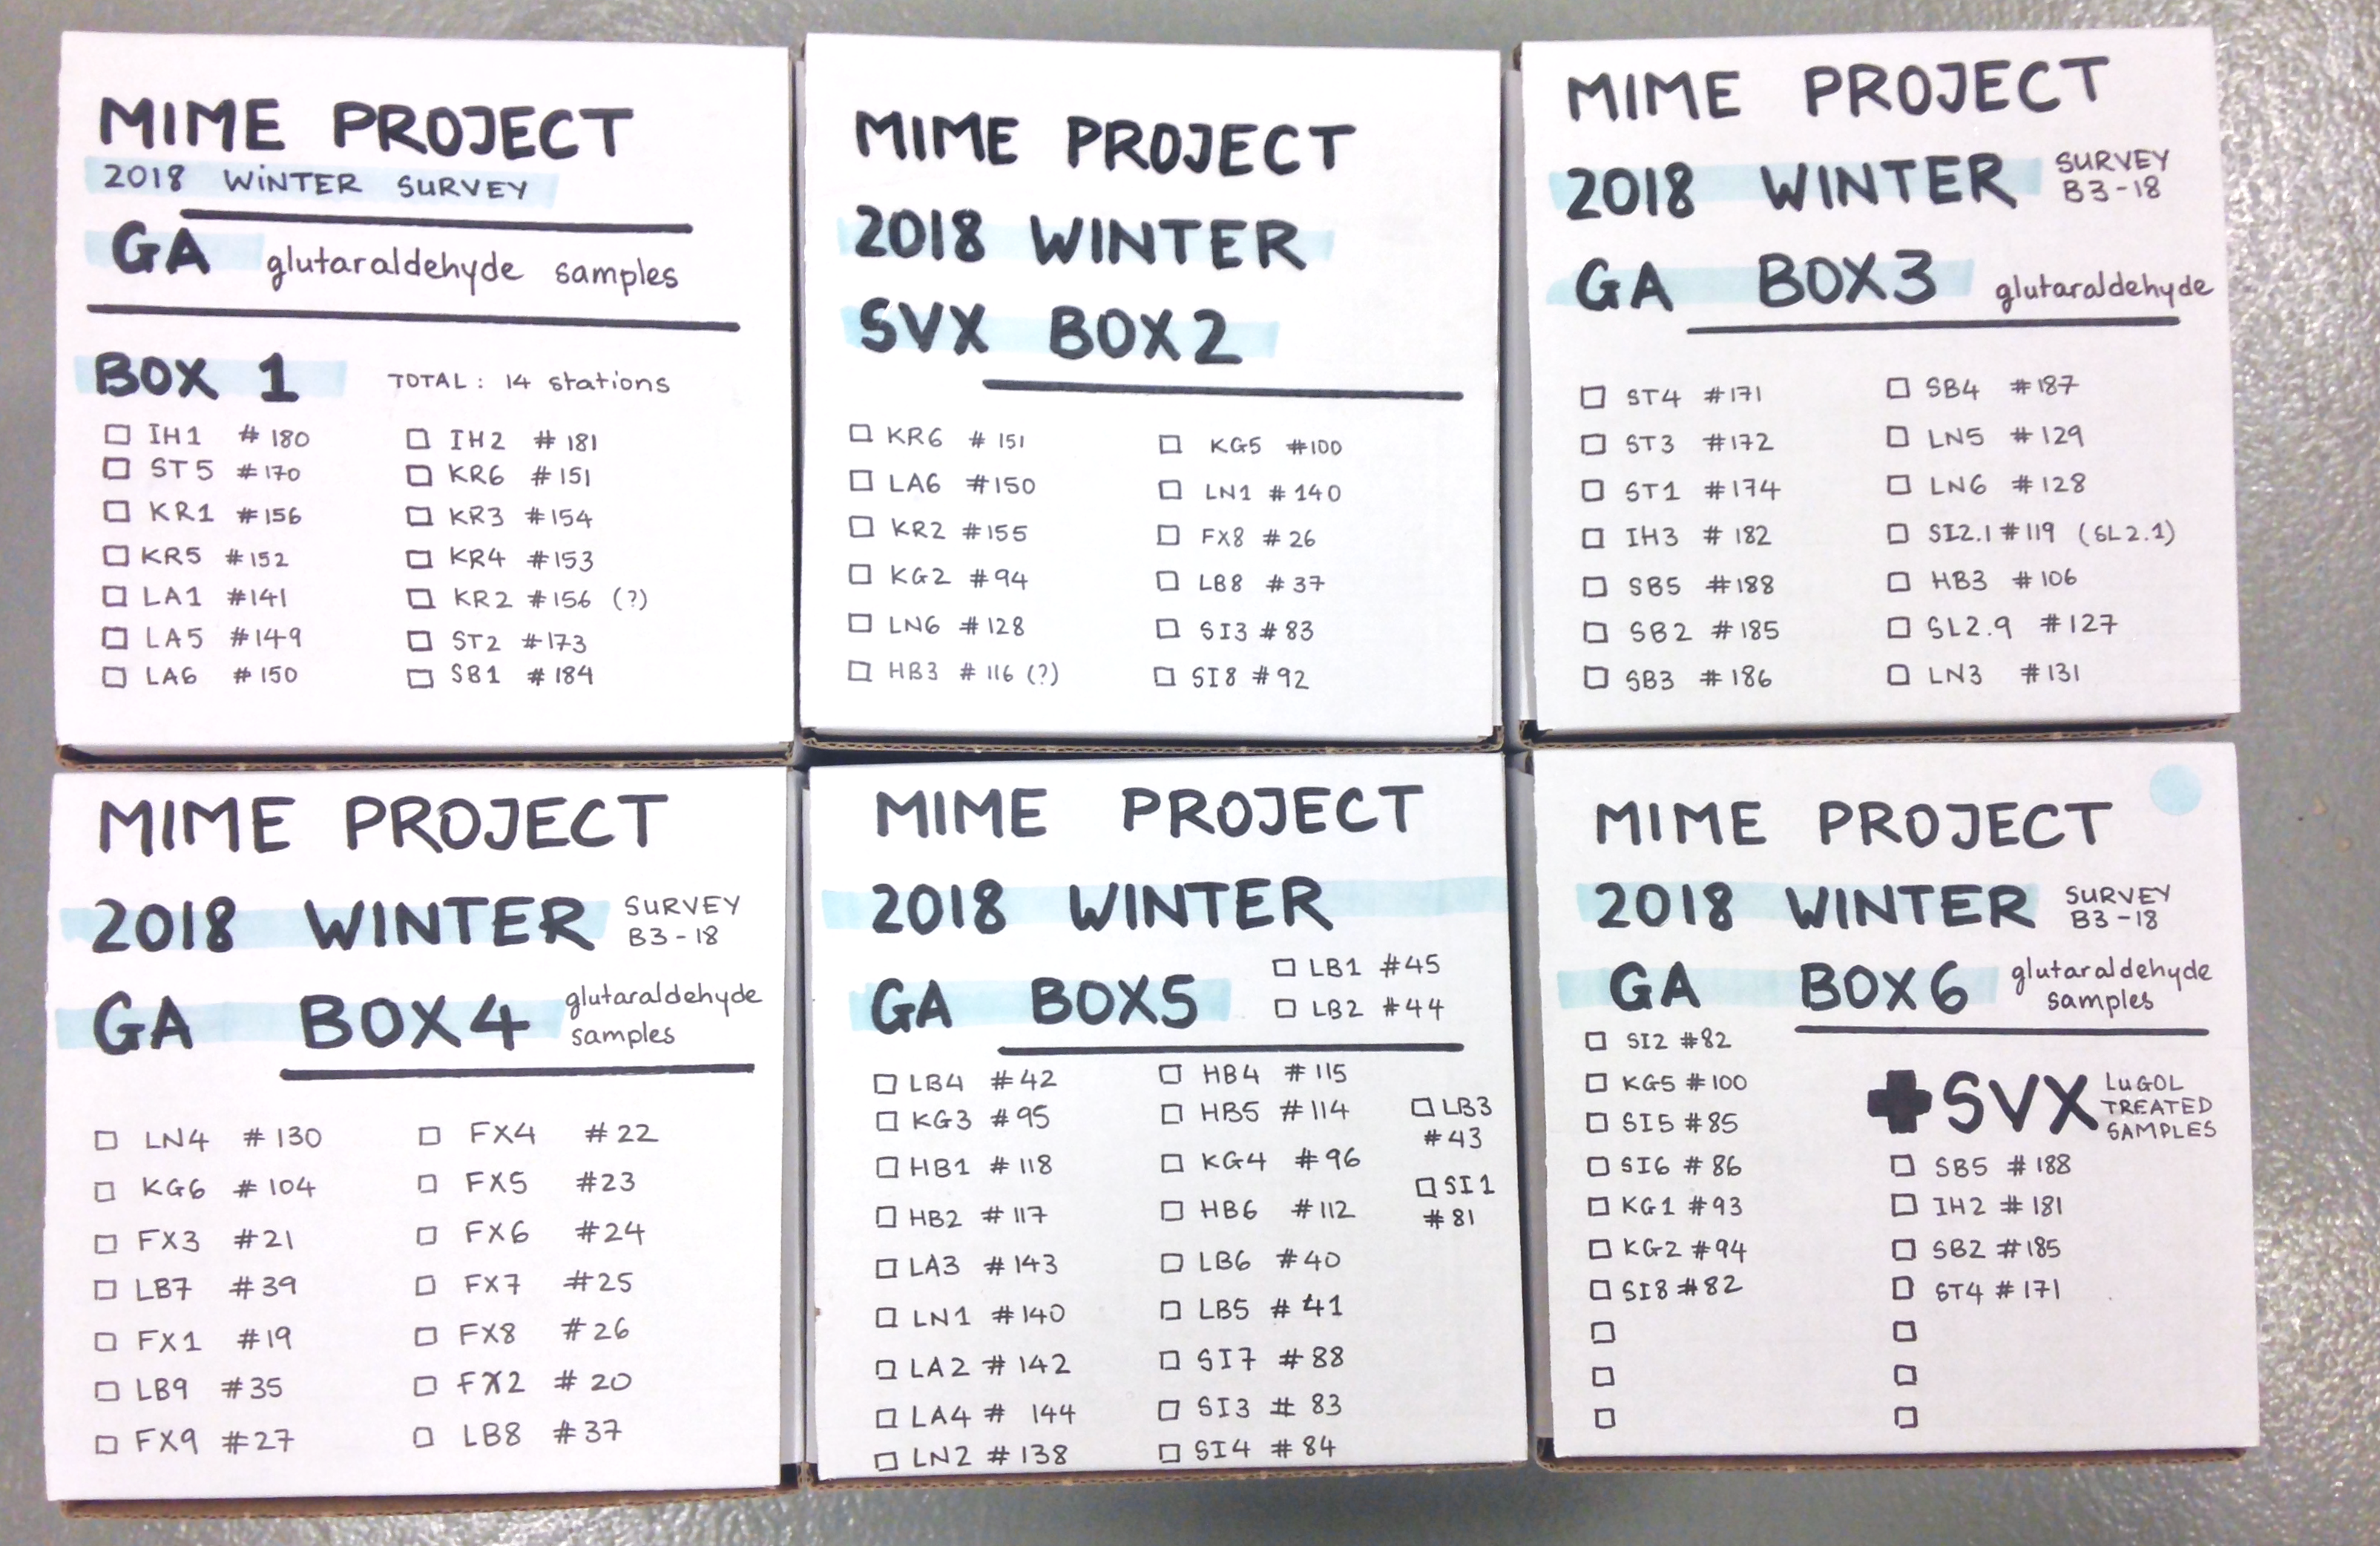
\includegraphics[width=\textwidth]{graphics/pic/20180313_boxes_freezer_winter_survey.png}
\end{figure}